\newpage
\section{Results}
\subsection{Sverdrup circulation}
The Sverdrup solution gave \autoref{fig:f_plane}--\ref{fig:sverdrup_u10}. One can in \autoref{fig:f_plane} see the result of the $f$-plane, which does not resemble the beta Sverdrup theory. Here the solution is symmetric, since there is no latitudinal asymmetry caused by the $\beta$-term. Furthermore, the solution is growing with time, due to the continuous input of wind energy. This is a growing geostrophic solution to the applied wind stress, and thus symmetric in the domain. However, an gyre can still be seen due to the consequence of the $y$-dependence on the wind stress. 

\begin{figure}[H]
    \centering    
    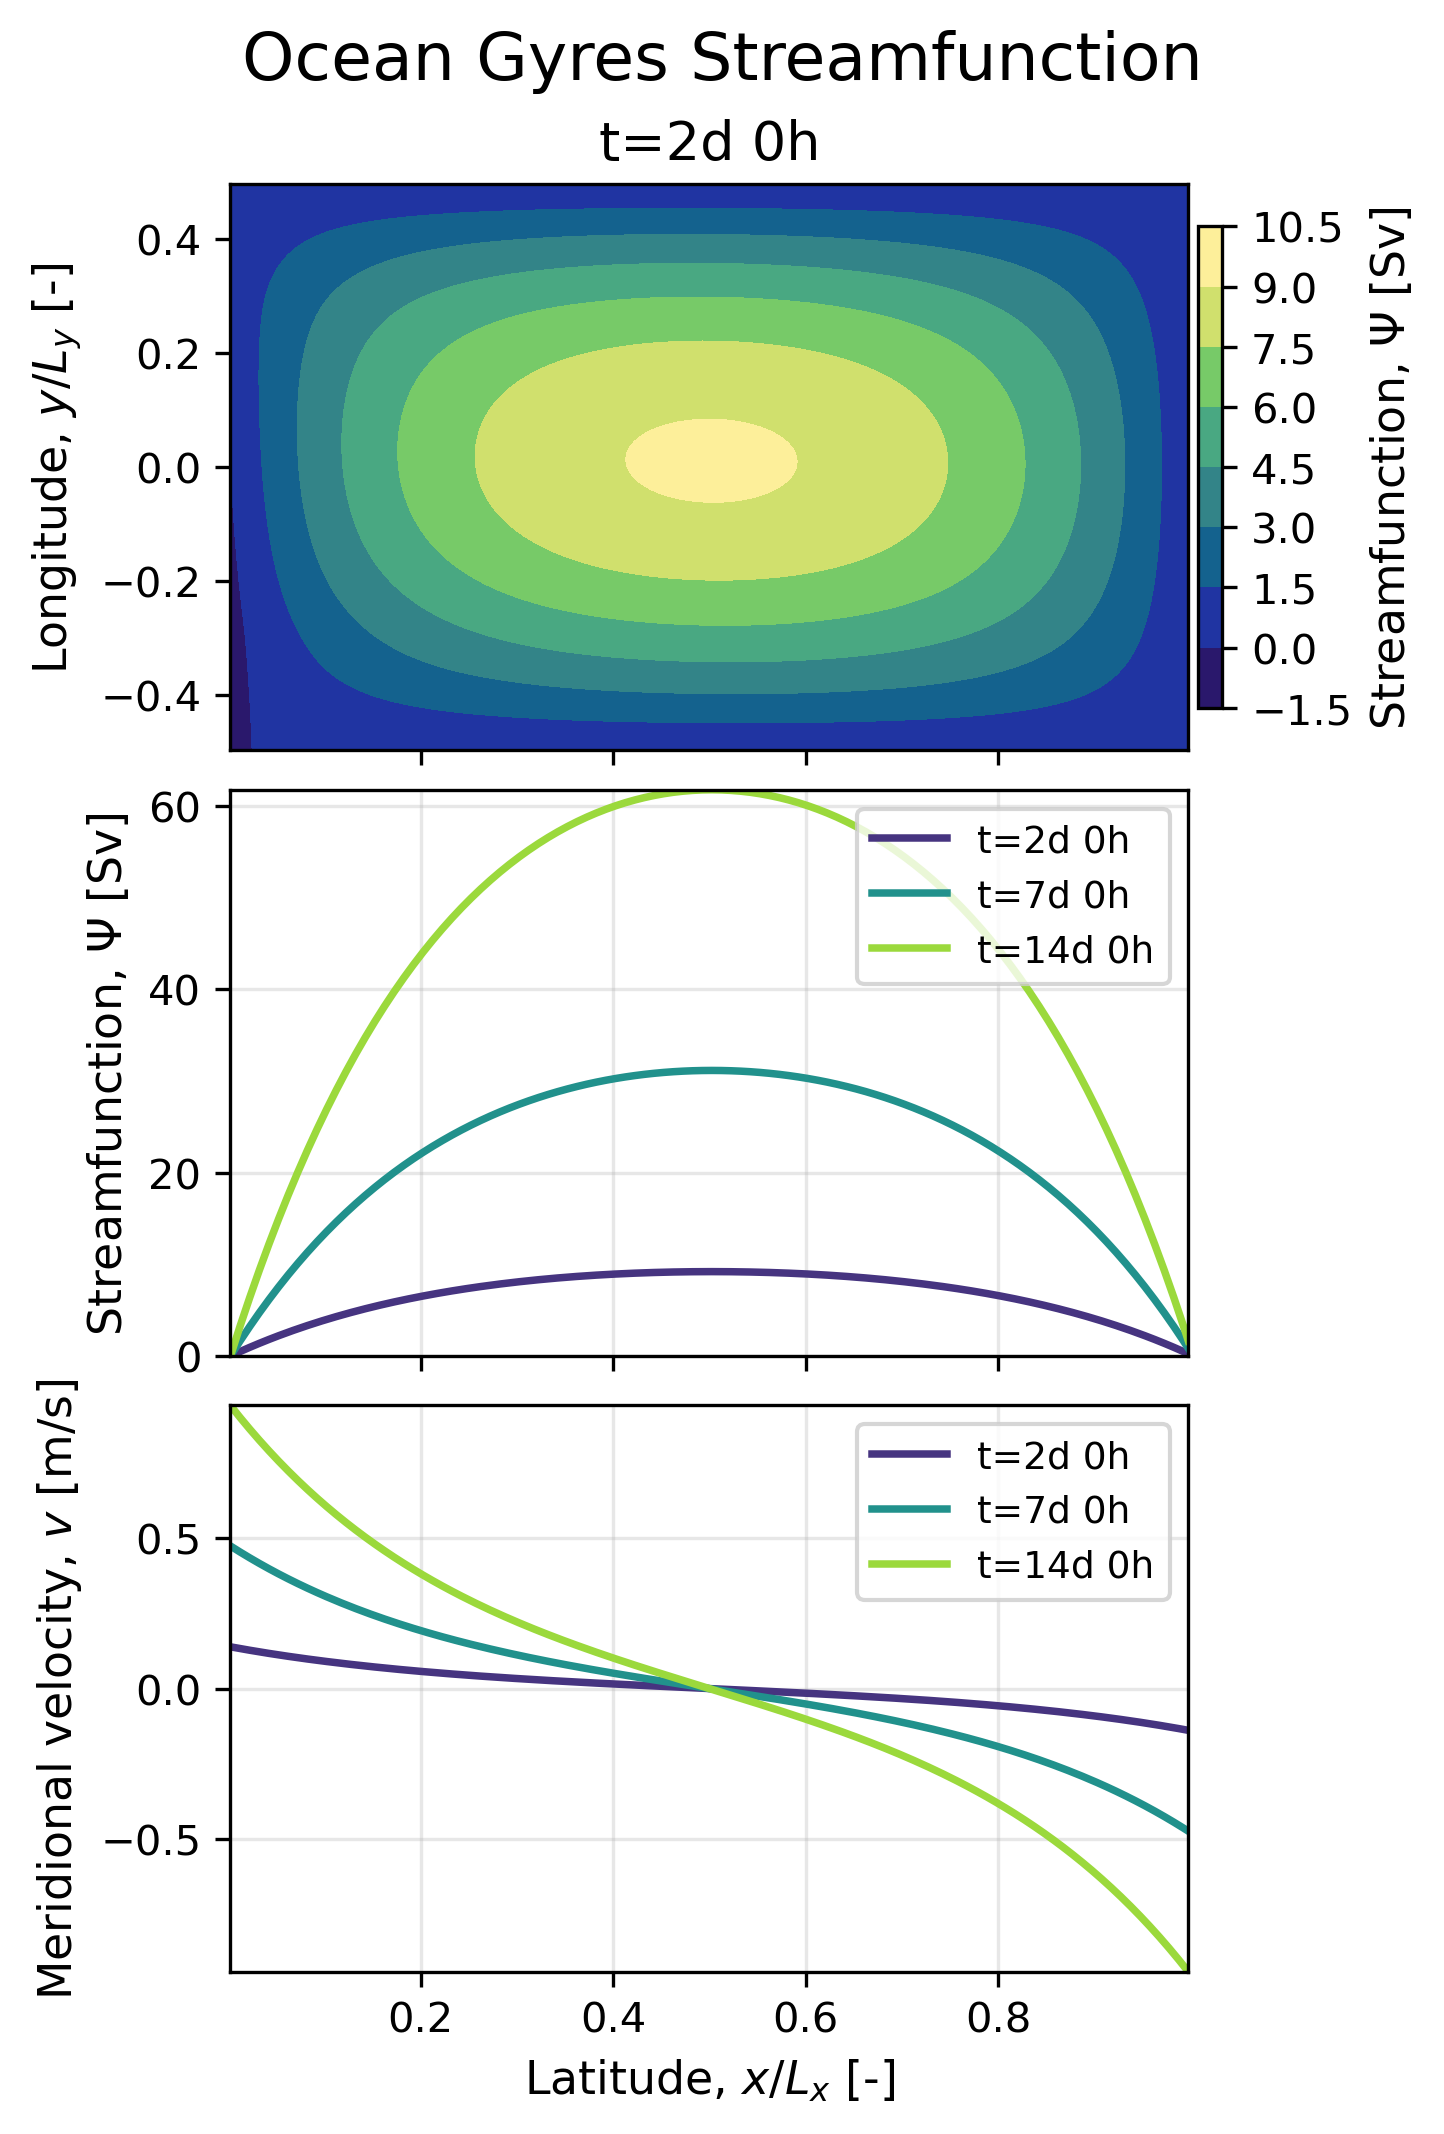
\includegraphics[height=0.63\textwidth]{../../plots/f_plane_vertical.png}
    \caption{Streamfunction for the no-viscosity $f$-plane, for different times.}
    \label{fig:f_plane}
\end{figure}

The introduction of the $\beta$-term gave \autoref{fig:sverdrup_u10}. One can observe Sverdrup like solution compared to \autoref{fig:f_plane}, due to the asymmetric beta effect (stronger $f$ northward and weaker southward) pushing the solution towards the western boundary. The mirror-symmetry is thus broken and a better Sverdrup solution is obtained. 

By increasing the wind stress one can observe linearly increases in the flux of the domain. This is reasonable since the wind stress is the forcing that drives this circulation. Thus, more forcing yields larger fluxes. Examining the slope, one sees larger southward velocities in the interior. Overall, one can see good agreement for the time-averaged result and the theory. Away from the western boundary the model and the theory align very good, but close to the western boundary they align very bad. 


\begin{figure}[H]
    \centering    
    
\includegraphics[height=0.63\textwidth]{../../plots/sverdrup_u10.png}
    \caption{Comparison of streamfunction for different wind stresses. The contours show the model result, while the solid red lines showcase the Sverdrup theory. The cross-sections of the streamfunction is at the center of the domain. The meridional wind velocity has been transformed into an Ekman-layer velocity, by assuming an Ekman depth of $\delta_\text{EK}=\SI{50}{\meter}$. The meridional velocity is thus the corresponding mass flux as if the domain is at rest and only the Ekman layer is moving. The time averaging was done between two days and eighty days.}
    \label{fig:sverdrup_u10}
\end{figure}

\begin{figure}[H]
    \centering    
    
\includegraphics[height=0.63\textwidth]{../../plots/sverdrup_vs_munk.png}
    \caption{This figure shows the effect of the Munk friction. The red lines are the theoretical Sverdrup and Munk solutions respectively.}
    \label{fig:sverdrup_vs_munk}
\end{figure}

\newpage
\subsection{Munk's theory}

The difference of including Munk viscosity gave \autoref{fig:sverdrup_vs_munk}. One can observe that the Munk theoretical results now include the western boundary current, in both the numerical and theoretical solution. Thus, the numerical solutions agrees better with the theoretical, compared to the Sverdrup solution. The largest distinction is the steady state convergence of the Munk model, which does not occur for the Sverdrup model. Observing the instantaneous relative error one can see a convergence towards lower errors for the Munk solution, while the same cannot be said for the Sverdrup solution. One thus needs to time average the Sverdrup result to obtain good values. One can observe that the time-averaged Sverdrup solution gives similar accuracy to the instantaneous Munk solution. However, to make a fair compression between the two models, the Munk solution was also time averaged.

Munk theory gave \autoref{fig:munk_a}. Increasing the viscosity coefficient $A$ can be seen to do two major things: broadening the western boundary current and thus also lowering the northward velocity. The location of the western boundary current can be observed to be precisely at the Munk layer $\delta_M$. Compared to the Sverdrup solution one observes better result in \autoref{fig:munk_a}, especially for the western boundary current.

\begin{figure}[H]
    \centering    
    
\includegraphics[height=0.63\textwidth]{../../plots/munk_a.png}
    \caption{Streamfunction for different values of the viscosity coefficient $A$. The contours show the model result, while the solid red lines showcases the theory. The resolution of the Munk depth is $\tfrac{\delta_M}{\Delta x}=[3.8, \ 4.9, \ 8.4]$, from left to right in the figure. The center domain zonal cross-sections show solid lines for the numerical model, while dashed lines represent Munk theory. The meridional wind velocity has again been transformed into an Ekman-layer velocity (as explained in \autoref{fig:sverdrup_u10}). The time-averaging was done between two days and eighty days.}
    \label{fig:munk_a}
\end{figure}

In \autoref{fig:atlantic_vs_pacific} one can observe the effect of increasing the domain width, while keeping $\Delta x$ constant. One can observe a larger flux for the North Pacific compared to the North Atlantic, although the meridional velocity is exactly the same in the two oceans (as seen from the slope of the streamfunctions). This also provides the larger domain with a faster western boundary current. 

\begin{figure}[H]
    \centering    
    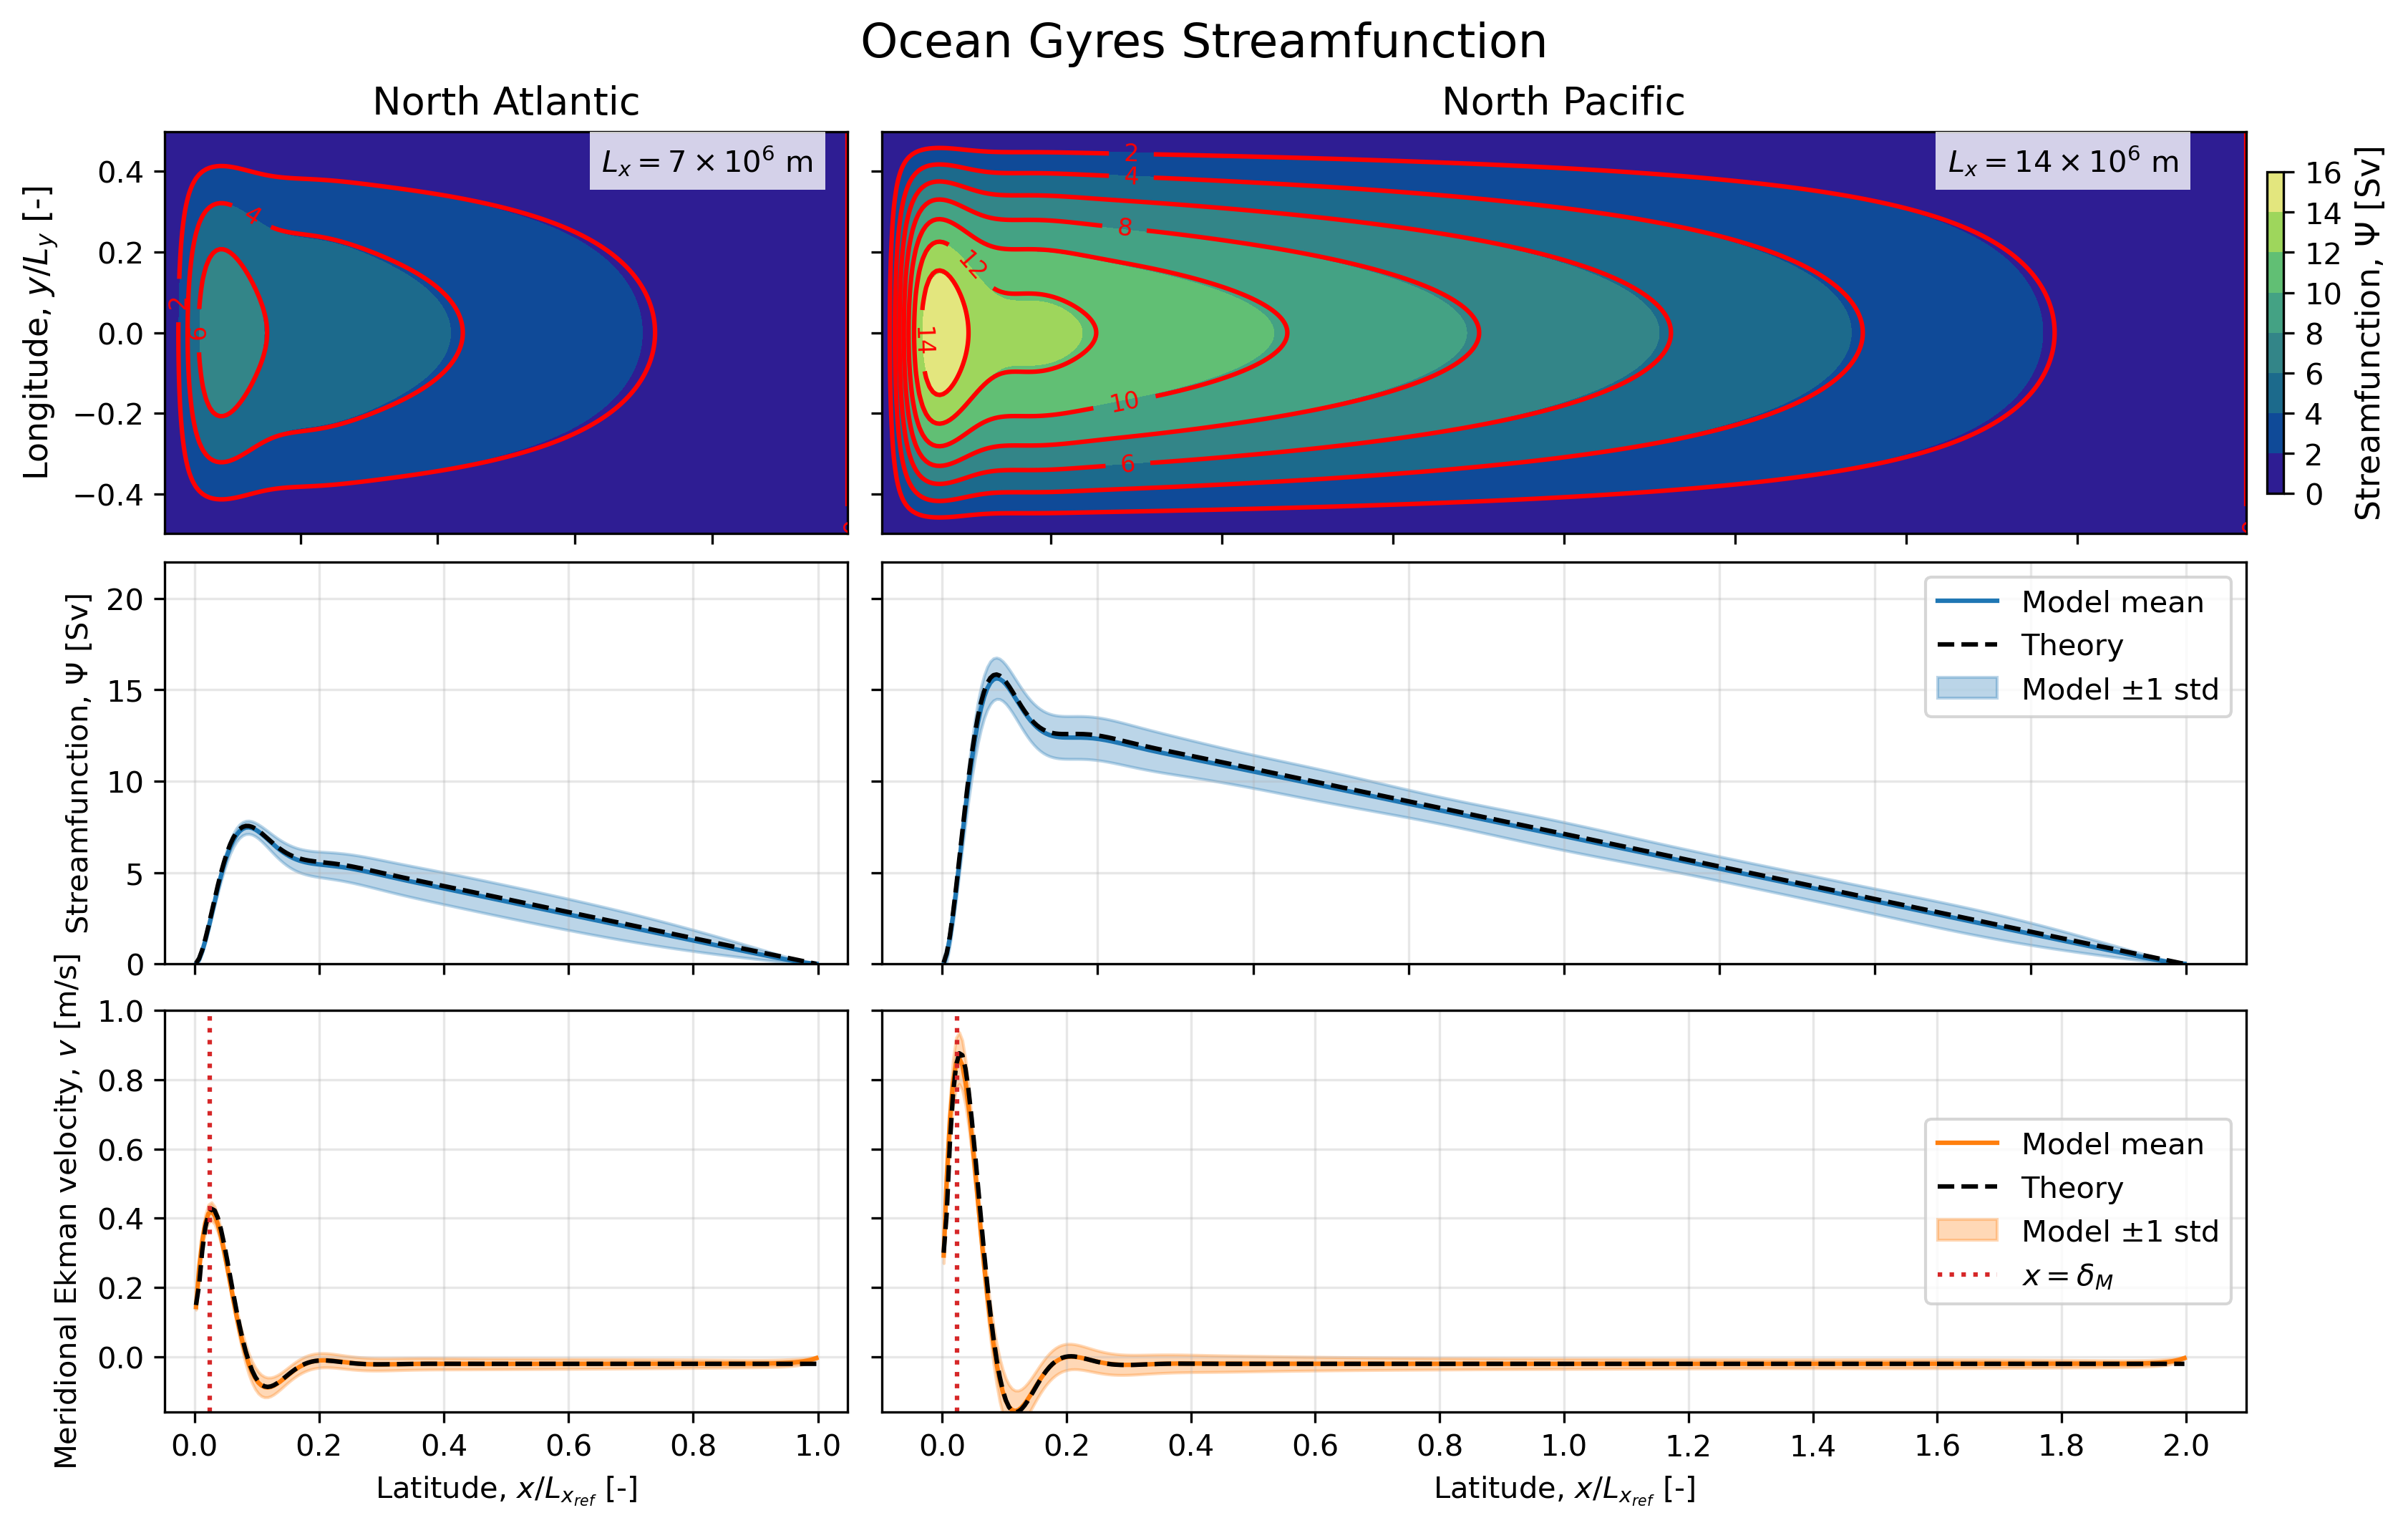
\includegraphics[height=0.63\textwidth]{../../plots/atlantic_vs_pacific_munk.png}
    \caption{Streamfunction for the viscosity configuration with varying domain size. The contours show the model result, while the solid red lines showcases the Munk theory. In the center domain cross-section, solid lines show the numerical model results, while dashed lines show theory. The meridional wind velocity has been transformed into an Ekman-layer velocity. The time averaging was done between two days and eighty days.}
    \label{fig:atlantic_vs_pacific}
\end{figure}


